
% This LaTeX was auto-generated from an M-file by MATLAB.
% To make changes, update the M-file and republish this document.

\documentclass{article}
\usepackage{graphicx}
\usepackage{color}

\sloppy
\definecolor{lightgray}{gray}{0.5}
\setlength{\parindent}{0pt}

\begin{document}

    
    
\subsection*{Contents}

\begin{itemize}
\setlength{\itemsep}{-1ex}
   \item Exercise 2
   \item Exercise 3
   \item Exercise 4
   \item Exercise 5
\end{itemize}


\subsection*{Exercise 2}

\begin{verbatim}
% Create two signals:
% (a) Create a length-12 vector representing an impulse 0 and 11.
delta1 = [1 zeros(1,11)];

% (b) Create a wave s1 with L = 80, A = 2, b = 0.08, and M = 20
s1 = Exercise1(80,2,0.08,20);
\end{verbatim}


\subsection*{Exercise 3}

\begin{verbatim}
% Use conv to convolve s1 and delta1, and plot the result using stem.
exercise3 = figure;
stem(conv(s1,delta1))
title('Exercise 3 - Convolution of s1 and delta1')
\end{verbatim}

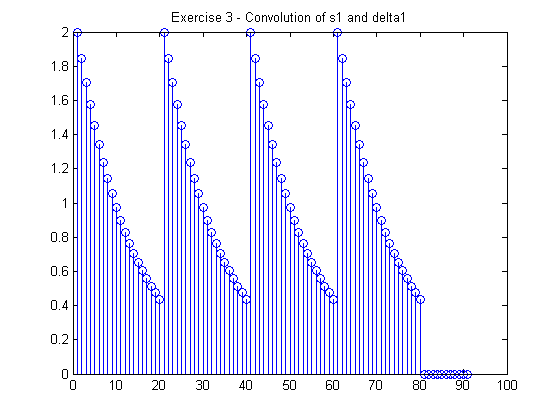
\includegraphics [width=4in]{Exercise2th5_01.png}


\subsection*{Exercise 4}

\begin{verbatim}
% Examine another convolution:
% (a) Create another vector of length 12 representing an impulse at 0 and 11.
delta2 = [1 zeros(1,10) 1];

% (b) Convolve delta2 with s1 and plot the result
exercise4 = figure;
stem(conv(s1,delta2))
title('Exercise 4 - Convolution of s1 and delta2')
\end{verbatim}

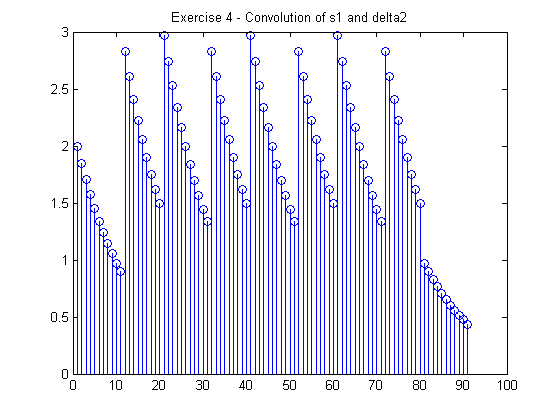
\includegraphics [width=4in]{Exercise2th5_02.png}


\subsection*{Exercise 5}

\begin{verbatim}
% Examine another type of impulse response:
% (a)Create a flat impulse response hn3 that is three points long and
% normalized by the length
hn3 = 1/3 * [ones(1,3)];

% (b) Convolve hn3 with s1
exercise5a = figure;
stem(conv(s1,hn3))
title('Exercise 5 - Convolution of hn3 and s1')

% (c) Increase the length of the impulse response to 5 and 10 and redo the
% convolution
hn5 = 1/5 * [ones(1,5)];
hn10 = 1/10 * [ones(1,10)];

exercise5c1 = figure;
stem(conv(s1,hn5))
title('Exercise 5 - Convolution of hn5 and s1')

exercise5c2 = figure;
stem(conv(s1,hn10))
title('Exercise 5 - Convolution of hn10 and s1')
\end{verbatim}

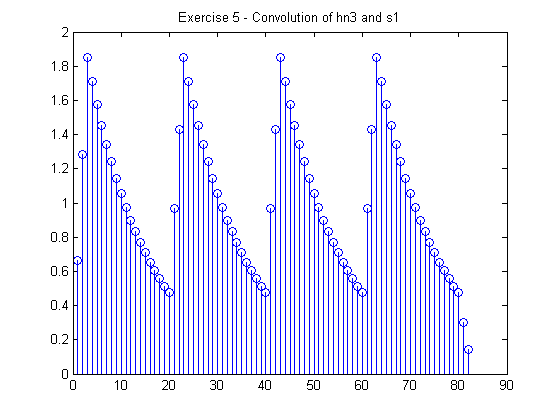
\includegraphics [width=4in]{Exercise2th5_03.png}

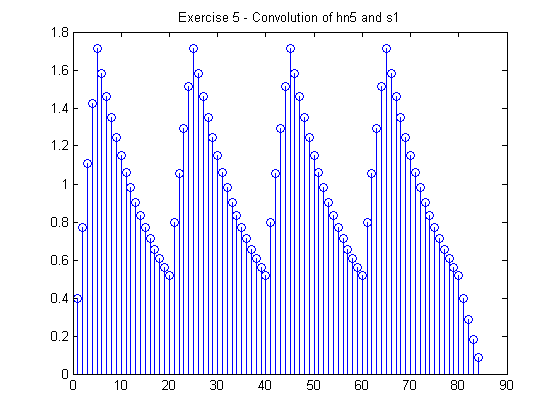
\includegraphics [width=4in]{Exercise2th5_04.png}

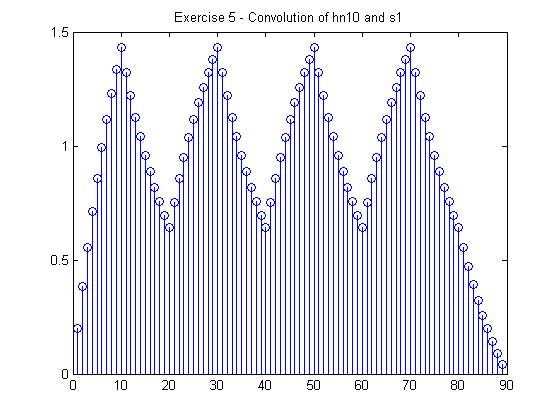
\includegraphics [width=4in]{Exercise2th5_05.png}



\end{document}
    
